%-----------------------------------------------------------------------------%
\chapter{\babSatu}
%-----------------------------------------------------------------------------%%

\section{Latar Belakang}
%-----------------------------------------------------------------------------%

Penyakit kulit merupakan salah satu masalah kesehatan masyarakat yang sangat signifikan secara global, termasuk di negara-negara tropis seperti Indonesia. Kondisi geografis dengan kelembaban tinggi, paparan sinar ultraviolet yang intens, dan tingkat kepadatan penduduk yang tidak merata menciptakan ekosistem yang mendukung prevalensi tinggi berbagai kondisi dermatologis. Menurut laporan \textit{Global Burden of Disease Study}, Indonesia tercatat berada pada peringkat ke-75 dari 195 negara dalam hal beban penyakit kulit secara global \citep{gbd2019}. Peringkat ini menempatkan Indonesia dalam kuartil atas negara-negara dengan beban dermatologis tertinggi.

Data Riset Kesehatan Dasar (Riskesdas) 2018 mencatat bahwa sekitar 9,4\% penduduk Indonesia atau setara dengan 25 juta jiwa mengalami keluhan penyakit kulit dan jaringan subkutan \citep{kemenkes2018laporan}. Angka tersebut menempatkan penyakit kulit sebagai penyebab keluhan terbanyak ketiga setelah gangguan pernapasan dan pencernaan dalam sistem kesehatan nasional. Data ini tetap relevan sebagai acuan mengingat belum ada pembaruan survei nasional berskala serupa untuk kategori penyakit kulit hingga saat ini. Meskipun sebagian besar penyakit kulit tidak fatal, sifatnya yang kronis menurunkan kualitas hidup secara signifikan melalui rasa gatal, nyeri, disabilitas ringan, hingga stigma sosial. Akumulasi dampak ini berkontribusi terhadap tingginya angka \textit{Years Lived with Disability} (YLD), indikator utama beban penyakit menurut WHO \citep{who2017}. Di wilayah dengan sanitasi rendah seperti beberapa daerah di Nusa Tenggara Timur dan Papua, penyakit kulit bahkan menjadi masalah endemik yang persisten.

Permasalahan ini diperparah oleh kesenjangan struktural dalam distribusi tenaga medis. Berdasarkan data Perhimpunan Dokter Spesialis Kulit dan Kelamin Indonesia (Perdoski) tahun 2022, Indonesia hanya memiliki sekitar 1.500 dokter spesialis kulit dan kelamin \citep{perdoski2022data}. Rasio ini menghasilkan perbandingan 1 dokter untuk setiap 180.000 penduduk, jauh dari standar ideal 1:20.000 yang direkomendasikan untuk layanan kesehatan yang memadai. Sebagian besar spesialis terkonsentrasi di kota besar, meninggalkan daerah rural dengan akses minimal. Kekurangan tenaga ahli ini membuka peluang strategis bagi sistem pendukung diagnosis berbasis kecerdasan buatan (AI) untuk membantu tenaga medis umum melakukan triase dan diagnosis awal yang lebih akurat. Ringkasan data beban penyakit kulit dan kapasitas layanan dermatologi di Indonesia disajikan pada Tabel \ref{tab:beban_penyakit}.

\begin{table}[H]
    \centering
    \caption{Beban Penyakit Kulit dan Kapasitas Layanan Dermatologi di Indonesia}
    \label{tab:beban_penyakit}
    \resizebox{\textwidth}{!}{%
    \begin{tabular}{|l|l|}
        \hline
        \textbf{Keterangan} & \textbf{Nilai} \\
        \hline
        Prevalensi Keluhan Kulit (Riskesdas 2018) & 9,4\% dari populasi ($\pm$ 25 juta jiwa) \\
        Peringkat Global Beban Penyakit Kulit (GBD 2019) & 75 dari 195 negara \\
        Jumlah Dokter Spesialis Kulit (Perdoski 2022) & $\pm$ 1.500 dokter \\
        Rasio Dokter Kulit : Penduduk & 1 : 180.000 \\
        Rasio Ideal (Target Kemenkes/WHO) & 1 : 20.000 \\
        \hline
    \end{tabular}%
    }
    \par\medskip
    \footnotesize Sumber: Diolah dari Riskesdas (2018), GBD (2019), dan Perdoski (2022)
\end{table}

Untuk mengatasi tantangan diagnosis pada kondisi keterbatasan data medis, paradigma \textit{Few-Shot Learning} (FSL) telah muncul sebagai solusi menjanjikan \citep{wang2020generalizing, liu2022meta}. FSL memungkinkan model untuk mengenali kategori penyakit baru dengan hanya menggunakan sedikit contoh (1-5 gambar), meniru kemampuan adaptasi manusia. Namun, metode FSL konvensional seringkali masih bersifat statis dalam memproses fitur, yang menyebabkan performa kurang optimal ketika menghadapi variasi visual yang tinggi antar pasien atau kondisi pencahayaan yang berbeda.

Sebagai upaya perbaikan, pendekatan \textit{Metric Learning} telah diadopsi secara luas dalam FSL untuk mempelajari ruang fitur di mana jarak geometris mencerminkan kemiripan semantik. Dalam paradigma ini, pendekatan berbasis \textit{attention} seperti \textit{Cosine Transformer} telah diperkenalkan sebagai \textit{baseline} yang kuat. Metode ini memanfaatkan mekanisme atensi untuk memfokuskan model pada fitur-fitur relevan dan menggunakan \textit{cosine similarity} untuk mengurangi dampak variasi skala fitur. Meskipun menawarkan peningkatan dibanding metode FSL standar, \textit{Cosine Transformer} masih memiliki kekurangan fundamental: mekanisme regularisasinya bersifat statis. Artinya, model menerapkan parameter regularisasi yang sama untuk setiap episode diagnosis, padahal tingkat kesulitan dan karakteristik visual setiap kasus bisa sangat bervariasi. Kekakuan ini membatasi kemampuan model untuk beradaptasi secara optimal pada kasus-kasus sulit atau data dengan \textit{noise} tinggi.

Merespons keterbatasan tersebut, penelitian ini mengusulkan metode \textbf{Dynamic VIC Few-Shot Learning}. Metode usulan ini mengembangkan \textit{baseline} yang ada dengan mengintegrasikan regularisasi statistik \textit{Variance-Invariance-Covariance} (VIC) yang diatur secara dinamis. Berbeda dengan pendekatan sebelumnya, metode ini mampu menyesuaikan bobot regularisasi secara adaptif berdasarkan karakteristik statistik dari setiap episode, serta memanfaatkan \textit{multihead attention} untuk menangkap fitur dari berbagai perspektif representasi.

Hingga saat ini, belum ada penelitian yang secara simultan menggabungkan regularisasi statistik adaptif, \textit{multihead attention}, dan pembobotan dinamis dalam arsitektur FSL untuk klasifikasi penyakit kulit tropis. Kebaruan pendekatan ini diharapkan dapat menghasilkan model yang lebih stabil menghadapi \textit{noise}, adaptif terhadap variasi kondisi pasien, dan akurat dalam mendeteksi penyakit langka meskipun jumlah sampel latihnya sangat sedikit.

Dari perspektif klinis, pengembangan model ini tidak hanya mengejar akurasi teknis, tetapi juga efisiensi dan keamanan. Model dirancang untuk menyeimbangkan performa diagnosis dengan kebutuhan komputasi yang ringan, sehingga memungkinkan implementasi masa depan di perangkat terbatas yang umum tersedia di Puskesmas.

Dalam penelitian ini, validasi arsitektur dilakukan menggunakan dataset publik standar yang dimodifikasi untuk mensimulasikan kondisi \textit{few-shot} dan ketimpangan kelas yang ekstrem. Penggunaan dataset ini bertujuan untuk memvalidasi efektivitas arsitektur usulan secara objektif sebelum tahap validasi klinis lanjutan.

Dengan menghadirkan pendekatan \textit{Dynamic VIC}, penelitian ini diharapkan tidak hanya memberikan kontribusi teoritis pada ranah \textit{Computer Vision}, tetapi menjadi langkah awal menuju pengembangan sistem diagnosis dermatologi berbantuan AI yang dapat diimplementasikan pada perangkat dengan sumber daya terbatas di fasilitas kesehatan primer.


%-----------------------------------------------------------------------------%
\section{Pertanyaan Penelitian}
%-----------------------------------------------------------------------------%

Secara ringkas, permasalahan utama yang diidentifikasi pada Bab 1 meliputi: (1) Keterbatasan jumlah data teranotasi dan ketimpangan kelas yang ekstrem pada kasus dermatologi, dan (2) Keterbatasan metode FSL \textit{baseline} yang masih bersifat statis dan kurang adaptif terhadap variasi kesulitan antar episode.

Berdasarkan latar belakang yang telah diuraikan, penelitian ini merumuskan pertanyaan penelitian utama sebagai berikut:

\begin{enumerate}
	\item Apakah arsitektur \textit{Dynamic VIC Few-Shot Learning} yang mengintegrasikan regularisasi statistik adaptif (Variance, Invariance, Covariance) mampu meningkatkan performa klasifikasi penyakit kulit dibandingkan metode \textit{baseline}, dan bagaimana kontribusi setiap komponen terhadap peningkatan tersebut?
\end{enumerate}


%-----------------------------------------------------------------------------%
\section{Hipotesis}
%-----------------------------------------------------------------------------%

Pada penelitian ini, penulis mengajukan hipotesis utama sebagai berikut:

\begin{itemize}
	\item $H_1$: Metode usulan \textit{Dynamic VIC Few-Shot Model} menghasilkan peningkatan performa yang signifikan (akurasi dan macro-F1) dibandingkan metode \textit{baseline} pada skenario data terbatas, di mana integrasi lengkap komponen VIC dan pembobotan dinamis memberikan kontribusi positif yang terukur terhadap stabilitas dan akurasi model.
	\item $H_0$: Metode usulan tidak menghasilkan peningkatan performa yang signifikan dibandingkan metode \textit{baseline}, atau komponen-komponen usulan tidak memberikan kontribusi yang berarti.
\end{itemize}


%-----------------------------------------------------------------------------%
\section{Tujuan Penelitian}
%-----------------------------------------------------------------------------%

Berikut beberapa tujuan penelitian yang ingin dicapai pada penelitian ini, antara lain:

\begin{enumerate}
	\item Mengembangkan arsitektur \textit{few-shot learning} berbasis Dynamic VIC yang mengintegrasikan komponen \textit{variance}, \textit{invariance}, dan \textit{covariance} dengan mekanisme \textit{attention} dinamis untuk klasifikasi penyakit kulit pada skenario data terbatas.
	
	\item Mengidentifikasi konfigurasi optimal komponen Dynamic VIC untuk klasifikasi penyakit kulit dengan data terbatas melalui studi ablasi komponen VIC.

	\item Mengevaluasi performa klasifikasi dan efisiensi komputasi model usulan (berdasarkan jumlah parameter dan waktu inferensi) dibandingkan dengan metode \textit{baseline} untuk memvalidasi kelayakan implementasi pada perangkat dengan sumber daya terbatas.

\end{enumerate}


%-----------------------------------------------------------------------------%
\section{Manfaat Penelitian}
%-----------------------------------------------------------------------------%

Penelitian ini diharapkan memberikan manfaat sebagai berikut. Dari segi ilmiah, penelitian ini mengusulkan kombinasi regularisasi VIC dengan mekanisme \textit{dynamic weighting} dan \textit{attention} dalam konteks \textit{few-shot learning} untuk klasifikasi citra medis, serta menyediakan analisis empiris komprehensif mengenai efektivitas setiap komponen dalam mengatasi keterbatasan data. Dari segi praktis, penelitian ini menunjukkan potensi pendekatan \textit{few-shot learning} untuk skrining penyakit kulit di layanan kesehatan primer dengan keterbatasan data berlabel, khususnya dalam konteks layanan kesehatan Indonesia yang menghadapi kesenjangan akses ke dokter spesialis.


%-----------------------------------------------------------------------------%
\section{Kontribusi Penelitian}
%-----------------------------------------------------------------------------%

Penelitian ini memberikan kontribusi ilmiah dan praktis yang disusun secara sistematis sebagai berikut:

\begin{enumerate}
	\item \textbf{Kontribusi Metodologis}: Mengusulkan arsitektur \textit{Dynamic VIC Few-Shot Model} yang mengintegrasikan secara simultan: (a) Regularisasi VIC (\textit{Variance-Invariance-Covariance}) untuk mencegah \textit{feature collapse}, (b) \textit{Multi-Head Cosine Attention} untuk ekstraksi fitur multi-skala, dan (c) \textit{Episode-Adaptive Dynamic Weighting} untuk adaptasi terhadap kesulitan episode. Kombinasi ini mengisi celah ilmiah di mana penelitian sebelumnya (berdasarkan SLR 2020--2025) hanya menerapkan komponen tersebut secara terpisah.
	
	\item \textbf{Kontribusi Empiris}: Menyajikan evaluasi komprehensif pada dataset benchmark (Omniglot, miniImageNet, CIFAR-FS, CUB, Yoga) dan dataset medis (HAM10000). Hasil eksperimen memberikan bukti empiris mengenai efektivitas regularisasi statistik dalam meningkatkan akurasi dan stabilitas prediksi pada skenario \textit{few-shot} dengan ketimpangan kelas tinggi.
	
	\item \textbf{Kontribusi Aplikatif}: Memvalidasi kelayakan penggunaan arsitektur ringan (Conv4 dengan $\approx$0,25 juta parameter) yang memiliki performa kompetitif namun jauh lebih efisien dibandingkan baseline. Hal ini mendukung potensi implementasi di fasilitas kesehatan primer (Puskesmas) dengan sumber daya komputasi terbatas.
	
	\item \textbf{Kontribusi Teknis}: Menyediakan implementasi kode berbasis PyTorch yang teroptimasi memori (\textit{mixed precision}, \textit{gradient checkpointing}) serta kerangka kerja evaluasi yang dapat direproduksi, yang tersedia untuk komunitas riset guna mendukung pengembangan lanjutan dalam dermatologi digital.
\end{enumerate}


%-----------------------------------------------------------------------------%
\section{Batasan Penelitian}
%-----------------------------------------------------------------------------%

Penelitian ini memiliki beberapa batasan yang perlu dicatat:

\begin{enumerate}
	\item Penelitian difokuskan pada klasifikasi penyakit kulit berbasis citra dermoskopik, tidak mencakup modalitas \textit{imaging} lain seperti \textit{clinical photography} atau \textit{multispectral imaging}.
	
	\item Evaluasi utama dilakukan pada dataset publik HAM10000 yang mayoritas berasal dari populasi Kaukasia (Eropa dan Oseania) dengan tipe kulit Fitzpatrick I--III. Penelitian ini belum mencakup pengujian ekstensif pada dataset lokal dengan karakteristik kulit tropis (Fitzpatrick IV--VI) karena keterbatasan ketersediaan data teranotasi yang siap pakai.
	
	\item \textbf{Keterbatasan Dataset Lokal Indonesia}: Pada penelitian ini, validasi masih berbasis dataset publik internasional yang mayoritas kulit terang. Konteks Indonesia hadir pada analisis latar belakang permasalahan dan motivasi penelitian, namun validasi langsung pada dataset lokal Indonesia dengan karakteristik kulit Fitzpatrick IV--VI menjadi pekerjaan lanjutan karena keterbatasan waktu dan ketersediaan data teranotasi yang memenuhi standar kualitas.
	
	\item Terdapat variabilitas perangkat dermoskopi di lapangan yang mungkin berbeda dengan standar kualitas citra pada dataset HAM10000. Penelitian ini belum menguji ketahanan model terhadap variasi perangkat keras yang ekstrem secara komprehensif.
	
	\item Penelitian ini tidak mencakup aspek \textit{deployment} aplikasi klinis maupun integrasi dengan sistem informasi kesehatan yang ada. Pengembangan aplikasi antarmuka pengguna dan integrasi sistem dibahas sebagai rekomendasi penelitian lanjutan pada Bab 5.
	
	\item Validasi klinis skala besar dengan dermatolog bersertifikat tidak termasuk dalam \textit{scope} penelitian ini. Hasil penelitian harus diinterpretasikan sebagai bukti konsep (\textit{proof-of-concept}) teknologi yang memerlukan validasi klinis lanjutan.

\end{enumerate}


%-----------------------------------------------------------------------------%
\section{Research Gap}
\label{sec:research_gap}
%-----------------------------------------------------------------------------%

Berdasarkan analisis literatur terkini, teridentifikasi beberapa kesenjangan penelitian utama yang menjadi motivasi studi ini:

\begin{enumerate}
    \item \textbf{Absennya Integrasi Regularisasi Statistik pada FSL Dermatologi}: Belum ada studi yang secara eksplisit menangani stabilitas representasi fitur melalui regularisasi statistik (VIC) untuk mencegah \textit{feature collapse} pada data dermatologi yang sangat tidak seimbang.
    
    \item \textbf{Keterbatasan Adaptabilitas Model Statis}: Metode yang ada umumnya menggunakan parameter regularisasi statis, yang tidak optimal untuk menangani variasi kesulitan antar episode diagnosis. \textbf{Kontribusi utama penelitian ini adalah pengembangan mekanisme \textit{Dynamic Weighting} yang secara adaptif menyesuaikan bobot regularisasi ($\lambda_{var}$, $\lambda_{cov}$) berdasarkan statistik episode saat runtime}---sebuah pendekatan yang belum pernah diterapkan dalam konteks FSL dermatologi.
    
\end{enumerate}

Posisi unik penelitian ini dapat divisualisasikan melalui diagram Venn yang ditunjukkan pada Gambar \ref{fig:venn_research_position}, yang menggambarkan irisan kontribusi dari tiga domain utama.

\begin{figure}[H]
    \centering
    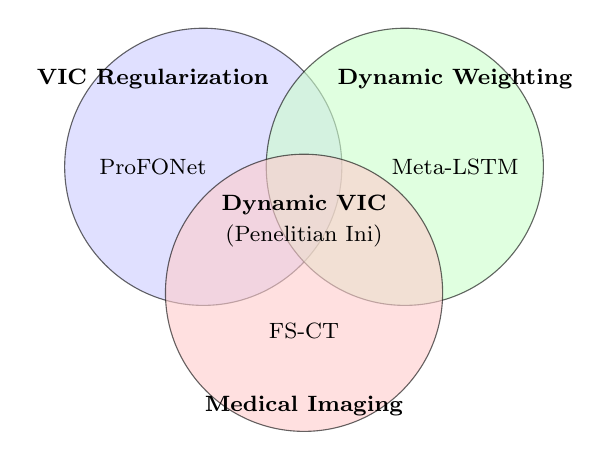
\begin{tikzpicture}[scale=0.8]
        % Venn diagram circles
        \def\radius{2.2cm}
        \def\sepA{-1.6cm}
        \def\sepB{1.6cm}
        \def\sepC{0cm}
        
        % Circle A - VIC Regularization (left)
        \draw[fill=blue!20, opacity=0.6] (\sepA,0.8cm) circle (\radius);
        \node at (\sepA-0.8cm,2.2cm) {\footnotesize \textbf{VIC Regularization}};
        \node at (\sepA-0.8cm,0.8cm) {\footnotesize ProFONet};
        
        % Circle B - Dynamic Weighting (right)
        \draw[fill=green!20, opacity=0.6] (\sepB,0.8cm) circle (\radius);
        \node at (\sepB+0.8cm,2.2cm) {\footnotesize \textbf{Dynamic Weighting}};
        \node at (\sepB+0.8cm,0.8cm) {\footnotesize Meta-LSTM};
        
        % Circle C - Medical Imaging (bottom)
        \draw[fill=red!20, opacity=0.6] (\sepC,-1.2cm) circle (\radius);
        \node at (\sepC,-3.0cm) {\footnotesize \textbf{Medical Imaging}};
        \node at (\sepC,-1.8cm) {\footnotesize FS-CT};
        
        % Center - Our contribution
        \node[font=\bfseries\footnotesize, text=black] at (0,0.2cm) {Dynamic VIC};
        \node[font=\footnotesize, text=black] at (0,-0.3cm) {(Penelitian Ini)};
    \end{tikzpicture}
    \caption{Diagram Venn Posisi Penelitian: Kontribusi unik \textit{Dynamic VIC Few-Shot Learning} terletak pada irisan ketiga domain---regularisasi VIC, pembobotan dinamis, dan pencitraan medis---yang belum pernah dieksplorasi secara bersamaan dalam literatur.}
    \label{fig:venn_research_position}
\end{figure}

Kesenjangan-kesenjangan ini dibahas lebih mendalam pada Bab 2.7. Penelitian ini bertujuan untuk menjembatani kesenjangan tersebut dengan mengembangkan model \textit{Dynamic VIC Few-Shot} yang secara spesifik dirancang untuk meningkatkan stabilitas representasi (menjawab Kesenjangan 1) dan beradaptasi secara dinamis (menjawab Kesenjangan 2), sebagaimana tercermin dalam rumusan Pertanyaan Penelitian.


%-----------------------------------------------------------------------------%
\section{Sistematika Penulisan}
%-----------------------------------------------------------------------------%

Laporan penelitian ini disusun dengan sistematika sebagai berikut:

\begin{itemize}
	\item \textbf{Bab 1 Pendahuluan} \\
	Bab ini menguraikan latar belakang penelitian, pertanyaan penelitian, hipotesis, tujuan penelitian, manfaat penelitian, kontribusi penelitian, batasan penelitian, dan sistematika penulisan.
	
	\item \textbf{Bab 2 Tinjauan Pustaka} \\
	Bab ini menyajikan kajian teoretis dan empiris mengenai klasifikasi citra medis, \textit{deep learning} dalam dermatologi digital, paradigma \textit{few-shot learning}, \textit{metric learning}, \textit{attention mechanism}, dan regularisasi representasi dengan fokus khusus pada pendekatan VIC.
	
	\item \textbf{Bab 3 Metodologi Penelitian} \\
	Bab ini menguraikan metodologi penelitian komprehensif yang mencakup desain penelitian, pengembangan algoritma, implementasi teknis, dan \textit{framework} evaluasi.
	
	\item \textbf{Bab 4 Hasil dan Analisis} \\
	Bab ini menyajikan hasil eksperimen, analisis performa, \textit{ablation studies}, dan visualisasi yang mendukung validasi hipotesis penelitian.
	
	\item \textbf{Bab 5 Kesimpulan dan Saran} \\
	Bab ini merangkum temuan utama penelitian, menyimpulkan kontribusi ilmiah, mengidentifikasi keterbatasan, dan memberikan rekomendasi untuk penelitian lanjutan.
\end{itemize}

